% As-built FSR-LM model stack (hymeko_lm). Standalone: pdflatex this file.
\documentclass[tikz,border=8pt]{standalone}
\usepackage{amsmath,amssymb}
\usetikzlibrary{arrows.meta,positioning,fit,backgrounds,calc}
\begin{document}
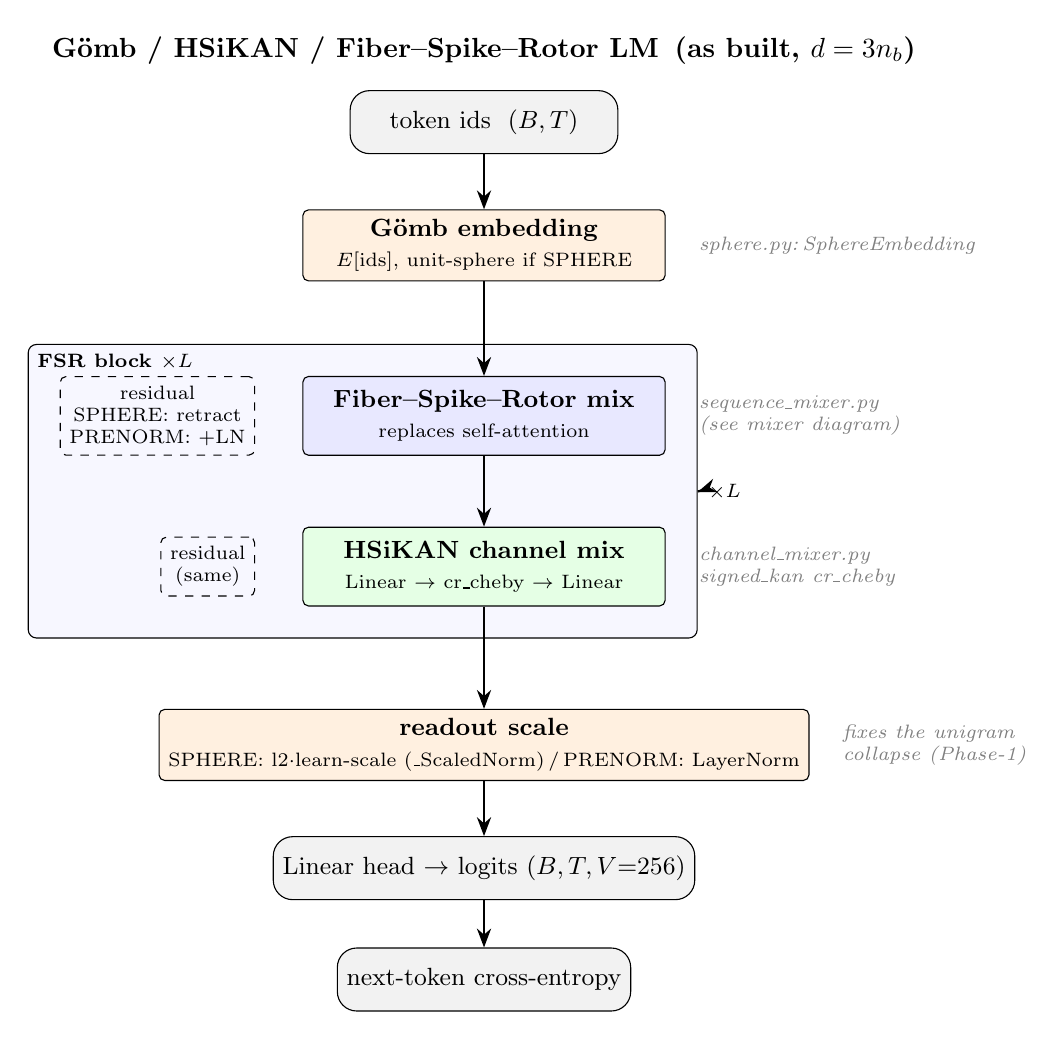
\begin{tikzpicture}[
  font=\small,>={Stealth[length=2.4mm]},
  io/.style={draw,rounded corners=7pt,fill=gray!10,align=center,minimum width=34mm,minimum height=8mm},
  gomb/.style={draw,rounded corners=2pt,fill=orange!12,align=center,minimum width=46mm,minimum height=9mm},
  mix/.style={draw,rounded corners=2pt,fill=blue!9,align=center,minimum width=46mm,minimum height=10mm},
  chan/.style={draw,rounded corners=2pt,fill=green!10,align=center,minimum width=46mm,minimum height=10mm},
  res/.style={draw,dashed,rounded corners=2pt,align=center,font=\scriptsize},
  ar/.style={->,thick},
  note/.style={font=\scriptsize\itshape,gray,align=left}
]
% spine
\node[io] (ids) {token ids\ \ $(B,T)$};
\node[gomb,below=7mm of ids] (emb) {\textbf{Gömb embedding}\\ \scriptsize $E[\text{ids}]$, unit-sphere if SPHERE};
\node[note,right=3mm of emb] {sphere.py:\,SphereEmbedding};

% block box
\node[mix,below=12mm of emb] (seq) {\textbf{Fiber--Spike--Rotor mix}\\ \scriptsize replaces self-attention};
\node[chan,below=9mm of seq] (chan) {\textbf{HSiKAN channel mix}\\ \scriptsize Linear $\to$ cr\_cheby $\to$ Linear};
\node[note,right=3mm of seq] {sequence\_mixer.py\\(see mixer diagram)};
\node[note,right=3mm of chan] {channel\_mixer.py\\ signed\_kan cr\_cheby};

% residual annotations
\node[res,left=6mm of seq] (r1) {residual\\ SPHERE: retract\\ PRENORM: $+$LN};
\node[res,left=6mm of chan] (r2) {residual\\ (same)};

% block grouping
\begin{scope}[on background layer]
  \node[draw,rounded corners=3pt,fill=blue!3,fit=(seq)(chan)(r1)(r2),inner sep=4mm] (blk) {};
\end{scope}
\node[font=\scriptsize\bfseries,anchor=north west] at (blk.north west) {FSR block $\times L$};

\node[gomb,below=13mm of chan] (fn) {\textbf{readout scale}\\ \scriptsize SPHERE: l2$\cdot$learn-scale\ (\_ScaledNorm)\,/\,PRENORM: LayerNorm};
\node[note,right=3mm of fn] {fixes the unigram\\collapse (Phase-1)};
\node[io,below=7mm of fn] (head) {Linear head $\to$ logits $(B,T,V{=}256)$};
\node[io,below=6mm of head] (loss) {next-token cross-entropy};

% arrows
\draw[ar] (ids) -- (emb);
\draw[ar] (emb) -- (seq);
\draw[ar] (seq) -- (chan);
\draw[ar] (chan) -- (fn);
\draw[ar] (fn) -- (head);
\draw[ar] (head) -- (loss);
% recurrence
\draw[ar,dashed] (blk.east) to[out=-20,in=20] node[right,note,black]{$\times L$} ($(blk.east)+(0,-0.01)$);

% title
\node[font=\bfseries,above=2mm of ids] {Gömb / HSiKAN / Fiber--Spike--Rotor LM \,(as built, $d=3n_b$)};
\end{tikzpicture}
\end{document}
